\documentclass[11pt,a4paper]{report}
%% For two-sided printing (for dead-tree output) comment previous line
%% and uncomment the next line
%\documentclass[11pt,a4paper,twoside,openright]{report}

\usepackage[utf8]{inputenc}

%% In general, the dissertation goes through several stages
%%
%% option       stage
%% -----------------------------
%% (no option)  text is in the preparation stage
%% juri         version for evaluation by committee
%% final        version for final submission (after acceptance)

%% Additional options for feupteses.sty
%%
%% option       Description
%% -----------------------------
%% portugues    titles, etc in portuguese
%% onpaper      links are not shown (for paper versions)
%% backrefs     include back references from bibliography to citation place
%% iso          format references according to ISO 690 standard

\usepackage[meic]{feupteses}
%\usepackage[meic,juri]{feupteses}
%\usepackage[meic,final]{feupteses}

%% Packages loaded by feupteses.sty:
%% url, setspace, makeidx, graphicx, xcolor, etc (see README)

%% Include here any other packages you need
\usepackage{indentfirst}
\usepackage{pgfgantt}
\usepackage{cleveref}
\usepackage{amssymb}
\usepackage{enumitem}

%% Use folder ``figures'' to keep all your figures
\graphicspath{{figures/}}

%% Use folder ``backmatter'' to keep all your bibliography files
\addbibresource{backmatter/bibliography.bib}

%%========================================
%% Start of document
%%========================================
\begin{document}

\title{IEC 61499 Compliant Web-based IDE for Function Block Design}
\author{Pedro da Cunha Teixeira e Faro Beirão}

%% Uncomment next line for date of submission
%\thesisdate{July 31, 2008}

\copyrightnotice{Pedro Beirão, 2026}

\supervisor{Supervisor}{Prof.\ Rui Pinto}

%% Comment committee stuff for final version, if not used
% \committeetext{Approved in oral examination by the committee:}
% \committeemember{President}{Prof.\ $<$Name of the Professor$>$}
% \committeemember{Referee}{Prof.\ $<$Name of the Professor$>$}
% \committeemember{Referee}{Prof.\ $<$Name of the Professor$>$}

%% uncomment next line to draw a line for handwritten signature if needed
%\signature

%% Specify cover logo (in folder ``figures'') if needed
% \logo{logo.pdf}

%% Uncomment next line for additional text below the author's name (front page)
%\additionalfronttext{$<$Additional text$>$}

\begin{Prolog}
  %% abstract.tex: abstract in PT and EN  (FEUP regulations)
%% -------------------------------------------------------
% TODO write abstract
\chapter*{Resumo}
Sistemas de Produção Ciber-Físicos \acs{CPPS} place increasing demands on the software tools used to design and operate distributed industrial control applications. The \textit{IEC 61499} standard provides a structured and event-driven function block model well suited to these environments, yet existing development tools remain predominantly desktop-based and poorly adapted to collaborative or remote workflows. This dissertation investigates whether modern web technologies can meaningfully address these limitations and proposes \textit{PTERO}, a remote web-based \ac{IDE} for the modelling, deployment and monitoring of \textit{IEC 61499}-compliant applications.

The developed architecture shifts heavy orchestration workloads from local workstations to a centralised middleware server. To resolve the collaborative friction inherent to traditional file-based workflows, the platform incorporates a collaboration layer driven by \acp{CRDT}, facilitating concurrent multi-user visual modelling.

The system was validated through performance benchmarks against \textit{4diac IDE}. The evaluation demonstrated that \textit{PTERO} substantially reduced configuration overhead and improved the collaboration capabilities of the system. Furthermore, a usability study confirmed the participants' perception of these improvements. Ultimately, this research proves that migrating to a web-based engineering paradigm successfully modernizes distributed industrial automation.

\acresetall %% to reset the acronym usage

\chapter*{Abstract}
\acp{CPPS} place increasing demands on the software tools used to design and operate distributed industrial control applications. The \textit{IEC 61499} standard provides a structured and event-driven function block model well suited to these environments, yet existing development tools remain predominantly desktop-based and poorly adapted to collaborative or remote workflows. This dissertation investigates whether modern web technologies can meaningfully address these limitations and proposes \textit{PTERO}, a remote web-based \ac{IDE} for the modelling, deployment and monitoring of \textit{IEC 61499}-compliant applications.

The developed architecture shifts heavy orchestration workloads from local workstations to a centralised middleware server. To resolve the collaborative friction inherent to traditional file-based workflows, the platform incorporates a collaboration layer driven by \acp{CRDT}, facilitating concurrent multi-user visual modelling.

The system was validated through performance benchmarks against \textit{4diac IDE}. The evaluation demonstrated that \textit{PTERO} substantially reduced configuration overhead and improved the collaboration capabilities of the system. Furthermore, a usability study confirmed the participants' perception of these improvements. Ultimately, this research proves that migrating to a web-based engineering paradigm successfully modernizes distributed industrial automation.

\acresetall %% to reset the acronym usage
 % the abstract
  %%% un-sdg.tex: UN Sustainable Development Goals (FEUP regulations)
%% -------------------------------------------------------

\chapter*{UN Sustainable Development Goals} \label{chap:UnitedNations}

The United Nations \acp{SDG} provide a global framework for achieving a better and more sustainable future for all.
It includes 17 goals\footnote{\url{https://sdgs.un.org/goals}} to address the world's most pressing challenges, including poverty, inequality, climate change, environmental degradation, peace, and justice.

This dissertation contributes to the development of accessible, collaborative and efficient software tooling for industrial automation systems. By lowering the barriers to developing and deploying \textit{IEC 61499}-compliant distributed control applications, this work supports the broader goals of sustainable industrial development and technological inclusivity. The specific Sustainable Development Goal addressed is:

\begin{description}
\item [SDG 8]
Promote sustained, inclusive and sustainable economic growth, full and productive employment and decent work for all
\item [SDG 9]
Build resilient infrastructure, promote inclusive and sustainable industrialization and foster innovation
\end{description}

\begin{center}
\begin{tabular}{|l|l|p{58mm}|p{52mm}|}
\hline
\textbf{SDG} & \textbf{Target} & \textbf{Contribution} & \textbf{Performance Indicators and Metrics} \\
\hline
\hline
    \multirow{4}{*}{8} & 8.2 & Elevating technological productivity by shifting industrial engineering tasks from fragmented local setups to integrated, cloud-native automated workflows. & Reduction in engineering setup time and configuration overhead during deployment tasks. \\
\hline
    \multirow{4}{*}{9} & 9.4 & Simplifying \textit{IEC 61499} deployment lowers the cost and effort of adopting modern industrial automation practices. & Reduction in development effort compared to existing tools, as measured by workflow comparison and user evaluation. \\
    \cline{2-4} & 9.b & Open, easily accessible tooling fosters industrial innovation in academic and research contexts where commercial tools are inaccessible. & Tool requires no per-user installation and is accessible across all major operating systems. \\
\hline
\end{tabular}
\end{center}
   % United Nations Sustainable Development Goals (SGD)
  \chapter*{Acknowledgements}
% \addcontentsline{toc}{chapter}{Acknowledgements}

I would like to express my gratitude to everyone that contributed to the realisation of this dissertation. I give my sincere thanks to:

My supervisor, Rui Pinto, for all confidence put onto me and the help throughout all the work.

Mariana Coimbra for her constant support, encouragement and feedback during this process. Her understanding and motivation were invaluable in the more demanding stages.

I would also like to thank my family and friends for their continuous support and encouragement, as well as everyone who contributed directly or indirectly to this project, whether through feedback, discussions, or assistance during testing and evaluation.

\vspace{10mm}
\flushleft{Pedro Beirão}
  % the acknowledgments
  %% This section is optional and can be removed
\cleardoublepage
\thispagestyle{plain}

\vspace*{8cm}

\begin{flushright}
   \textsl{``Programming is not a zero-sum game. Teaching something to a fellow programmer doesn't take it away from you. I'm happy to share what I can, because I'm in it for the love of programming.''} \\
\vspace*{1.5cm}
John Carmack
\end{flushright}
    % initial quotation if needed
  \cleardoublepage
  \pdfbookmark[0]{Table of Contents}{contents}
  \tableofcontents
  \cleardoublepage
  \pdfbookmark[0]{List of Figures}{figures}
  \listoffigures
  \cleardoublepage
  \pdfbookmark[0]{List of Tables}{tables}
  \listoftables
  \cleardoublepage
  \pdfbookmark[0]{List of Listings}{listings}
  \renewcommand{\lstlistlistingname}{List of Listings}
  \lstlistoflistings
  \chapter*{List of Acronyms}
% Print the list of acronyms
\chaptermark{LIST OF ACRONYMS}

%% sort acronym entries manualy yourself

%% only the acronyms used in the text will be printed

\begin{acronym}[ASCII] % The longest acronym goes here (for alignment)
  \acro{CPPS}{Cyber-Physical Production Systems}
  \acro{CRDT}{Conflict-free Replicated Data Type}
  \acro{FBD}{Function Block Diagram}
  \acro{ICS}{Industrial Control Systems}
  \acro{IDE}{Integrated Development Environment}
  \acro{PLC}{Programmable Logic Controller}
  \acro{RTE}{Runtime Environment}
  \acro{SOA}{Service-Oriented Architectures}
  \acro{UI}{User Interface}
\end{acronym}

\end{Prolog}

\StartBody

\chapter{Introduction} \label{chap:intro}

\section{Context} \label{sec:ae1}

\ac{CPPS} are complex systems that integrate physical processes with digital technologies to optimise production processes. Several software engineering approaches and technologies are utilised in the development and operation of \ac{CPPS}. One of such approaches is \ac{FBD}. \ac{FBD} is a graphical programming language used in industrial automation and control systems. \ac{FBD} uses graphical function blocks to represent the logic and control of a system. The function blocks are connected in a network to form a control program. One of the benefits of \ac{FBD} is that it provides a visual representation of the control logic, which can be easier to understand and debug than traditional textual programming languages. \ac{FBD} is also modular, which means that function blocks can be reused in multiple programs, reducing development time and improving code maintainability. Also, \ac{FBD} is often used in conjunction with \acp{PLC} to control machinery and processes in manufacturing and other industrial applications. \ac{FBD} programs can be created and edited using specialised software tools that allow for the creation and manipulation of function blocks.

Several methods and tools are used in \ac{FBD}, including the IEC 61499 standard. As IEC 61499 supporting tools, there are \acp{RTE} and \acp{IDE}. While \acp{RTE} enables the execution of Function Blocks compliant with the standard, \acp{IDE} are used to design, create, and deploy Function Block pipelines into the Edge layer of a \ac{CPPS}.

These \acp{IDE} offer features and tools that facilitate the development, testing, and deployment of IEC 61499-compliant control systems. They provide graphical editors for creating function block diagrams, simulation capabilities, and additional functionalities to streamline the development process. However, despite being increasingly popular, there aren’t many web-based \acp{IDE} specifically designed for IEC 61499.

\section{Motivation} \label{sec:ae2}

The evolution of \ac{CPPS} has increased the demand for flexible and intelligent control solutions capable of integrating physical processes with digital technologies. \ac{FBD} and the IEC 61499 standard offer a structured, modular approach to building such distributed automation systems. To fully leverage these benefits, development tools must evolve alongside industrial needs, supporting more accessible, collaborative, and scalable workflows.

\section{Problem} \label{sec:ae3}

Existing IEC 61499 development environments are predominantly desktop-based and lack modern capabilities such as remote access, real-time collaboration, and seamless integration with cloud or edge infrastructures. These limitations hinder efficient development, maintenance, and deployment of control applications within distributed \ac{CPPS}. As a result, current tools fall short in supporting the flexibility, scalability, and interconnectedness required by modern industrial automation systems.

\section{Research Questions} \label{sec:ae4}

This research seeks to investigate how modern web technologies can be leveraged to enhance the development, deployment, and operation of IEC 61499-compliant systems. This study is guided by the following main research question:
\begin{quote}
How can web-based \acp{IDE} enhance the development, deployment, and collaboration processes for IEC 61499 applications in distributed \ac{CPPS}, addressing the limitations of traditional desktop-based environments?
\end{quote}
To further refine the scope, the following sub-questions are proposed:
\begin{itemize}
  \item What architectural and technological mrequirements must be considered when designing a web-based \acp{IDE} for IEC 61499?
  \item In what ways do web-based \acp{IDE} improve collaboration, accessibility, and scalability compared to existing desktop tools?
\end{itemize} % Introduction
\chapter{Literature Review} \label{chap:ch2}

This chapter reviews prior work related to IEC 61499-based development, \ac{CPPS}, and web-based \acp{IDE}. The goal is to identify how current tools support distributed automation and where existing gaps justify the development of a web-based solution.

\section{Methodology} \label{sec:lr2}
A systematic literature review approach was adopted, the objective was to collect, screen, and analyze studies addressing IEC 61499 development tools, \ac{CPPS}, and web-based engineering environments.

\subsection{Search and Selection}
The search was conducted in \textit{ScienceDirect}, \textit{Scopus} and others using combinations of the following terms:

\begin{quote}
(\texttt{"IEC 61499"} OR \texttt{"FBD"}) AND (\texttt{"web-based"} OR \texttt{"IDE"}) AND (\texttt{"CPPS"})
\end{quote}

\section{Related Work} \label{sec:lr3}
Recent studies explore cloud-native automation and containerized function block execution \cite{Sorokin2022,Lyu2024}, yet most solutions remain constrained by traditional architectures. Emerging web-based IDE prototypes, such as early 4diac Web IDE developments \cite{Rohat2014}, show promise in accessibility and scalability but lack maturity and full IEC 61499 compliance.

 % Literature review
\chapter{State of the Art} \label{chap:ch3}

This chapter provides a comprehensive analysis of the current landscape regarding development environments for \ac{CPPS} and the IEC 61499 standard. It categorizes existing solutions into traditional desktop-based environments and emerging web-based engineering tools while identifying the key technological enablers that facilitate the migration of \ac{FBD} to the web.

\section{Development Ecosystem} \label{sec:sota_iec61499}

Currently, the development ecosystem is dominated by desktop-based \acp{IDE}. These tools are typically monolithic applications installed locally on engineering workstations.

\subsection{Open-Source}
The most prominent open-source implementation is the Eclipse 4diac framework. It consists of the 4diac IDE (based on the Eclipse framework) and the 4diac FORTE (a run-time environment), althought it can also use different \acp{RTE} like DINASORE.

This IDE is very feature rich at the cost of significant system resources and increased complexity which make it more difficult to use. It relies on the heavyweight Eclipse Rich Client Platform.

\subsection{Commercial}
The commercial side is dominated by EcoStruxure Automation Expert, ISaGRAF Workbench and other monolithic desktop based environments, usually with a built-in proprietary \ac{RTE}. This makes them often very complete production ready tools, but they are not very flexible and not the best fit for many needs.

\section{Evolution of Web-Based Engineering Tools} \label{sec:sota_web_tools}

The software engineering domain has seen a massive shift from desktop \acp{IDE} to cloud-native environments. This trend is now influencing the domain of \ac{ICS}. Recent studies have proposed \ac{SOA} to integrate IEC 61499 with cloud layers, yet the engineering tools themselves remain largely desktop-bound \cite{Siqueira2021}.

\subsection{Web-Based IDEs in Software Development}
In general software development, tools like Visual Studio Code have started offering web-based counterparts to their desktop applications in search of a more flexible user experience.

\section{Gap Analysis} \label{sec:sota_gap}

Current IEC 61499 tools face significant limitations that hinder modern \ac{CPPS} development:

\begin{itemize}
    \item \textbf{Platform Dependency:} Existing solutions are monolithic desktop applications, lacking the accessibility and portability of web-based environments.

    \item \textbf{Resource Intensity:} Current options are heavyweight and complex, creating a high barrier to entry compared to modern agile tooling.

    \item \textbf{The Web Gap:} Despite industry trends, there is currently no mature, lightweight web interface for \ac{FBD}, leaving \ac{ICS} engineering behind the curve of cloud-native software development.
\end{itemize} % State of the art
\chapter{Solution} \label{chap:solution}

\section{Approach}
% TODO This is the time where you describe your approach How you expect to solve the problem and justify it! Refer to requirements, limitations, identified gaps in the literature, improvements over others work, etc.


\section{Methods}

\subsection{Introduction}
% TODO State the purpose of the chapter and why the chosen methodology is appropriate for addressing the research question.
 % Proposed Solution
\chapter{Prototype Development}

To be able to prove the proposed solution is viable and will successfully address the gap identified, a prototype needs to be developed and afterwards validated. % TODO add a bit more here

% \section{Technology Selection}
% Firstly some decisions need to be made to choose the most appropriate technologies to support this work.

\section{Runtime Environment}
Out of all \acp{RTE} compatible with \textit{IEC 61499}, this prototype will focus on supporting \textit{DINASORE} (Dynamic INtelligent Architecture for Software and MOdular REconfiguration). It is much less complex than others, making it ideal for a proof of concept \ac{IDE}. As an open-source project, \textit{DINASORE} can be freely inspected and studied, which is particularly valuable in a research and prototyping context where flexibility is prioritised over real-time performance guarantees. This ease of study rules out the use of commercial \acp{RTE} like \textit{EcoStruxure Automation Expert's "dPAC"} and \textit{ISaGRAF Runtime}. Other open-source \acp{RTE} were considered, but none was as well-suited as \textit{DINASORE}. \textit{4diac FORTE} for example was way too extensive and complicated to be able to easily study it's source code.
% TODO maybe talk about the use of python both in dinasores code and the fbs code

\begin{figure}[h!]
  
\includegraphics[width=0.5\linewidth]{dinasore-logo.png}
  \caption{\textit{DINASORE} logo}
  \label{fig:dinasore-logo}
\end{figure}


\section{Server}
The design begins by setting up a server that will serve the \ac{IDE} interface as a webpage, store and manage all the data and handle communication with the \acp{RTE}. Taking into account the features we plan on implementing, \textit{JavaScript} running on \textit{Node.js} were chosen due to the extensive library ecosystem. For real-time collaboration we will need a library to run in both the server and the frontend, since \textit{JavaScript} runs natively in the browser, it further reinforces that it should also be used in the server. The library choice will be explained in depth in \Cref{sec:real-time-collaboration}, proving the previous train of thought.

Being the middleware, there are 4 different types of network communications that the server will need to handle, each with it's own requirements:

\begin{itemize}
  \item \textbf{Serve webpage}: Communicates via \textit{GET} requests to deliver the \textit{html}, \textit{css} and \textit{js} files that make up the \ac{IDE} interface.
  \item \textbf{Real-Time Collaboration}: Constant atomic updates via a library.
  \item \textbf{Requested deployment}: A team member sends a \textit{POST} request, that tells the server to deploy.
  \item \textbf{Deployment sockets}: Communicates via sockets with each \ac{RTE} to send commands and receive the corresponding responses.
\end{itemize}

\begin{figure}[h!]
  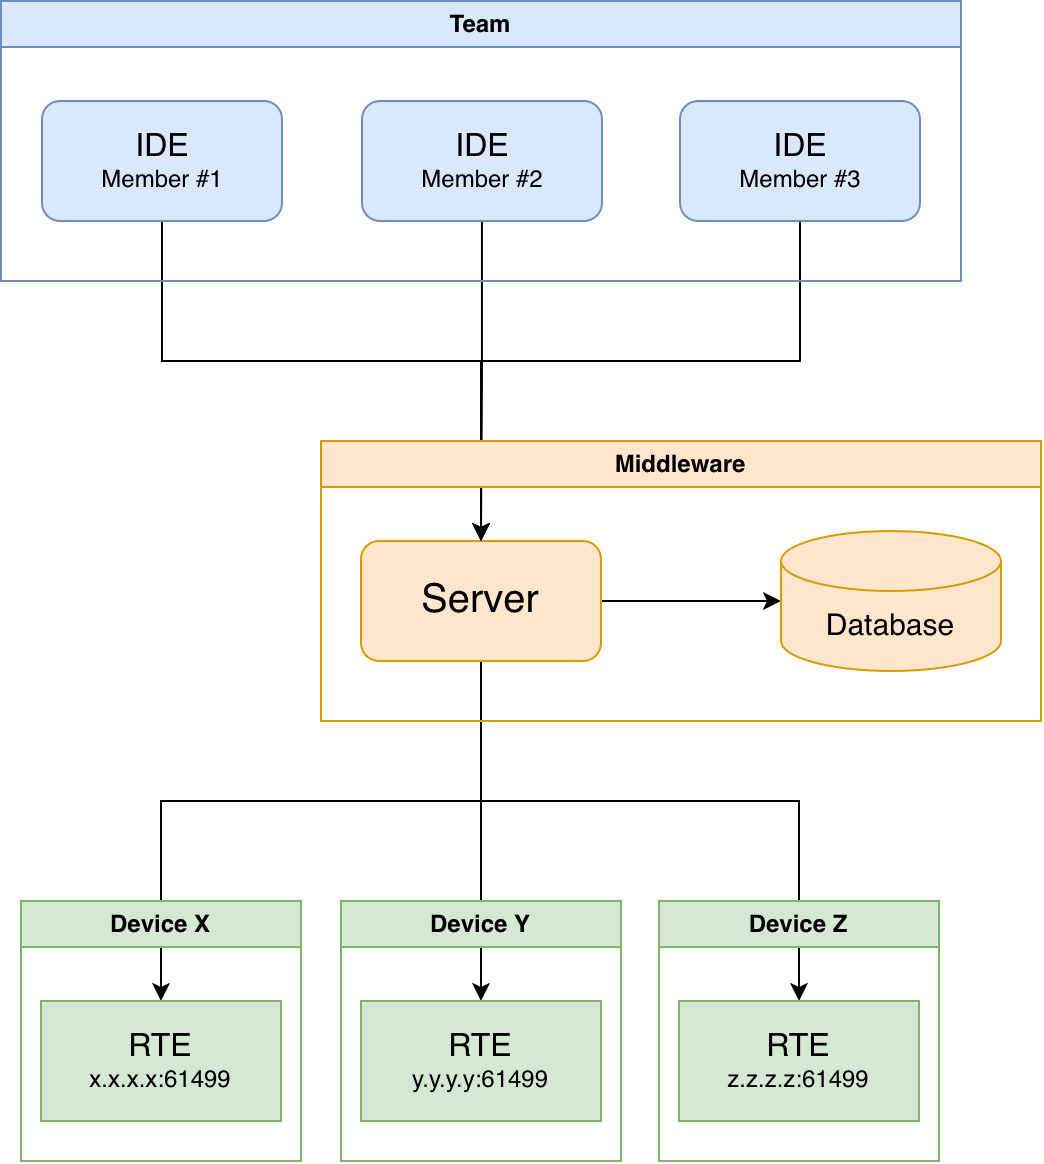
\includegraphics[width=1\linewidth]{ide-server-rte.jpg}
  \caption{Communication through the Middleware}
  \label{fig:ide-server-rte}
\end{figure}

\section{Frontend}
The frontend is the \ac{UI} that will be used to create and modify the \ac{FBD} programs. It consists of a 3 views.

\subsection{Devices Configuration}

\subsection{Function Blocks Editor View}

\subsection{Graph View}



\section{Real-Time Collaboration} \label{sec:real-time-collaboration}


\section{Deployment}
\subsection{Deployment Console}
 % Prototype Development
\chapter{Results and Analysis}
% TODO validate results
 % Results and analysis
\chapter{Conclusions}
% TODO talk about the main contributions of this work
% TODO mention further improvements
% TODO mention future work
% TODO mention what other tools can learn from this
 % Conclusion

\PrintBib

%% comment next 2 commands if numbered appendices are not used
\appendix
\chapter{Implementation} \label{app:implementation}

\section{Function Block Files}

\begin{lstlisting}[language=XML, caption={Example \textit{xml} definition of a function block}, label={lst:fb-xml}]
<FBType Name="NEW_FB_1">
  <InterfaceList>
    <EventInputs>
      <Event Name="INIT" Type="Event"/>
      <Event Name="READ" Type="Event">
        <With Var="VARIABLE_1"/>
        <With var="VARIABLE_2"/>
        <With var="VARIABLE_3"/>
      </Event>
    </EventInputs>
    <EventOutputs>
      <Event Name="INIT_O" Type="Event"/>
      <Event Name="READ_O" Type="Event">
        <With Var="DATA_1"/>
      </Event>
    </EventOutputs>
    <InputVars>
      <VarDeclaration Name="VARIABLE_1" Type="STRING"/>
      <VarDeclaration Name="VARIABLE_2" Type="REAL"/>
      <VarDeclaration Name="VARIABLE_3" Type="INT"/>
    </InputVars>
    <OutputVars>
      <VarDeclaration Name="DATA_1" Type="STRING"/>
    </OutputVars>
  </InterfaceList>
</FBType>
\end{lstlisting}


\begin{lstlisting}[language=Python, caption={Example \textit{Python} code of a function block}, label={lst:fb-py}]
class NEW_FB_1:
  def __init__(self):
    pass

  def schedule(self, event_name, event_value, variable_1, variable_2, variable_3):
    if event_name == "INIT":
      return [event_value, None, ""]

    elif event_name == "READ":
      return [None, event_value, ""]
\end{lstlisting}

\section{Synchronisation}

\begin{lstlisting}[language=JSON, caption={Sync configuration}, label={lst:sync-config}]
{
  master-fbs-path: 'sync/fbs',
  dinasores: [
    {
      address: 'x.x.x.x',
      port: 22,
      username: 'root',
      password: 'dinasore',
      dinasore-path: '/root/dinasore'
    },
    {
      address: 'y.y.y.y',
      port: 22,
      username: 'root',
      password: 'dinasore',
      dinasore-path: '/root/dinasore'
    }
  ]
}
\end{lstlisting}

\section{Communication} \label{app:implementation:communication}

\begin{lstlisting}[language=Python, caption={build\_message() in Python}, label={lst:build-message-py}]
def build_message(message_payload, configuration_name):
  # build the first part of the header
  hex_input = '{:04x}'.format(len(configuration_name))
  second_byte = int(hex_input[0:2], 16)
  third_byte = int(hex_input[2:4], 16)
  response_len = struct.pack('BB', second_byte, third_byte)
  response_header_1 = b''.join([b'\x50', response_len])

  # build the second part of the header
  hex_input = '{:04x}'.format(len(message_payload))
  second_byte = int(hex_input[0:2], 16)
  third_byte = int(hex_input[2:4], 16)
  response_len = struct.pack('BB', second_byte, third_byte)
  response_header_2 = b''.join([b'\x50', response_len])

  # join the 3 parts
  response = b''.join([response_header_1, configuration_name, response_header_2, message_payload])
  return response
\end{lstlisting}

\begin{lstlisting}[language=JavaScript, caption={build\_message() in JavaScript}, label={lst:build-message-js}]
function build_message(message_payload, configuration_name) {
  const configBuffer = Buffer.from(configuration_name, 'utf-8');
  const messageBuffer = Buffer.from(message_payload, 'utf-8');

  // Header 1: [0x50][len_hi][len_lo]
  const header1 = Buffer.alloc(3);
  header1[0] = 0x50;
  header1.writeUInt16BE(configBuffer.length, 1);

  // Header 2: [0x50][len_hi][len_lo]
  const header2 = Buffer.alloc(3);
  header2[0] = 0x50;
  header2.writeUInt16BE(messageBuffer.length, 1);

  return Buffer.concat([
    header1,
    configBuffer,
    header2,
    messageBuffer
  ]);
}
\end{lstlisting}

\section{Send Messages} \label{app:send-messages}
First we need to send the two commands in \Cref{lst:deploy-setup} to every device. A \texttt{QUERY} request and a \texttt{CREATE} request that will create a \textit{EMB\_RES} resource which will be automatically connected to the \textit{INIT} port of all other function block nodes to initialize them. Both these commands will have an empty configuration name, as \textit{EMB\_RES} has not been created yet and therefore cannot be bounded to.

\begin{lstlisting}[language=XML, caption={Setup deployment commands}, label={lst:deploy-setup}]
<Request Action="QUERY" ID="0">
  <FB Name="*" Type="*"/>
</Request>

<Request Action="CREATE" ID="1">
  <FB Name="EMB_RES" Type="EMB_RES"/>
</Request>
\end{lstlisting}

Next, depending on which commands are mapped to each machine, we \texttt{CREATE} all the mapped nodes and \texttt{WRITE} the initial input values with the commands in \Cref{lst:deploy-create-nodes}. The configuration name in these and all following commands will be "\textit{EMB\_RES}" as they need to be bound to it in order to be initialised and ran.

\begin{lstlisting}[language=XML, caption={\texttt{CREATE} nodes deployment commands}, label={lst:deploy-create-nodes}]
<Request Action="CREATE" ID="2">
  <FB Name="SENSOR_SIMULATOR" Type="SENSOR_SIMULATOR"/>
</Request>

<Request Action="WRITE" ID="3">
  <Connection Destination="SENSOR_SIMULATOR.OFFSET" Source="12"/>
</Request>

<Request Action="CREATE" ID="4">
  <FB Name="MOVING_AVERAGE" Type="MOVING_AVERAGE"/>
</Request>

<Request Action="WRITE" ID="5">
  <Connection Destination="MOVING_AVERAGE.WINDOW" Source="5"/>
</Request>
\end{lstlisting}

Then the connections are created between the mapped nodes. A \texttt{Source} a \texttt{Destination} must be provided, with the format \texttt{"NODE\_NAME.SLOT\_NAME"}, using the commands in \Cref{lst:deploy-create-links}.

\begin{lstlisting}[language=XML, caption={\texttt{CREATE} links deployment commands}, label={lst:deploy-create-links}]
<Request Action="CREATE" ID="6">
  <Connection Destination="SENSOR_SIMULATOR.READ_0" Source="MOVING_AVERAGE.RUN"/>
</Request>

<Request Action="CREATE" ID="7">
  <Connection Destination="SENSOR_SIMULATOR.VALUE" Source="MOVING_AVERAGE.VALUE"/>
</Request>
\end{lstlisting}

Finally the \texttt{START} command in \Cref{lst:deploy-start} can be issued, which will request for the start of the program execution. For this command the configuration name used will also be "\textit{EMB\_RES}" as it is this resource that will begin the execution of the program.

\begin{lstlisting}[language=XML, caption={\texttt{START} deployment command}, label={lst:deploy-start}]
<Request Action="START" ID="8"/>
\end{lstlisting}

After each request is sent, a response will be returned by the \textit{DINASORE}. It is important for the \ac{IDE} to listen for these responses and only send the next request once the response corresponding to the previous request is received. The responses have the format shown in \Cref{lst:deploy-response}. The \texttt{ID} of the response will be the same of the associated request. The format of the responses is the same as the requests and the configuration name that is used is empty.

\begin{lstlisting}[language=XML, caption={\texttt{Response} after a deployment command is sent}, label={lst:deploy-response}]
<Response ID="8"/>
\end{lstlisting}

\section{Watch} \label{app:watch}
Note in \Cref{lst:deploy-create-watch} that the \texttt{ID} is reset after deploying.

\begin{lstlisting}[language=XML, caption={\texttt{CREATE} watches after deploying}, label={lst:deploy-create-watch}]
<Request ID="0" Action="CREATE">
  <Watch Source="SENSOR_SIMULATOR.VALUE" Destination="*" />
</Request>

<Request ID="1" Action="CREATE">
  <Watch Source="MOVING_AVERAGE.VALUE_MA" Destination="*" />
</Request>
\end{lstlisting}

After creating the watches we can send a request to receive the values using the command in \Cref{lst:deploy-read-watch}. This will return the response in \Cref{lst:deploy-watch}, which by parsing the values, allows the prototype to display them in the \textit{Graph View}.

\begin{lstlisting}[language=XML, caption={Request to \texttt{READ} watches}, label={lst:deploy-read-watch}]
<Request ID="2" Action="READ">
  <Watches/>
</Request>
\end{lstlisting}

\begin{lstlisting}[language=XML, caption={Response to \texttt{READ} watches}, label={lst:deploy-watch}]
<Response ID="2">
	<Watches>
		<Resource name="EMB_RES">
			<FB name="SENSOR_SIMULATOR">
				<Port name="VALUE">
					<Data value="13.75" />
				</Port>
			</FB>
			<FB name="MOVING_AVERAGE">
				<Port name="VALUE">
					<Data value="13.3" />
				</Port>
			</FB>
		</Resource>
	</Watches>
</Response>
\end{lstlisting}

\chapter{Usability Validation Website} \label{app:validation-website}
The website used for usability validation was hosted at \href{https://ptero.pedro-beirao.eu}{https://ptero.pedro-beirao.eu}, and consisted of an instructions page with the steps required to recreate the \textit{Test Application} from \Cref{sec:test-application} and the \ac{IDE} frontend itself. The \Cref{fig:appendix-1,fig:appendix-2,fig:appendix-3,fig:appendix-4} preserve the state of the website during evaluation.

\begin{figure}[H]
  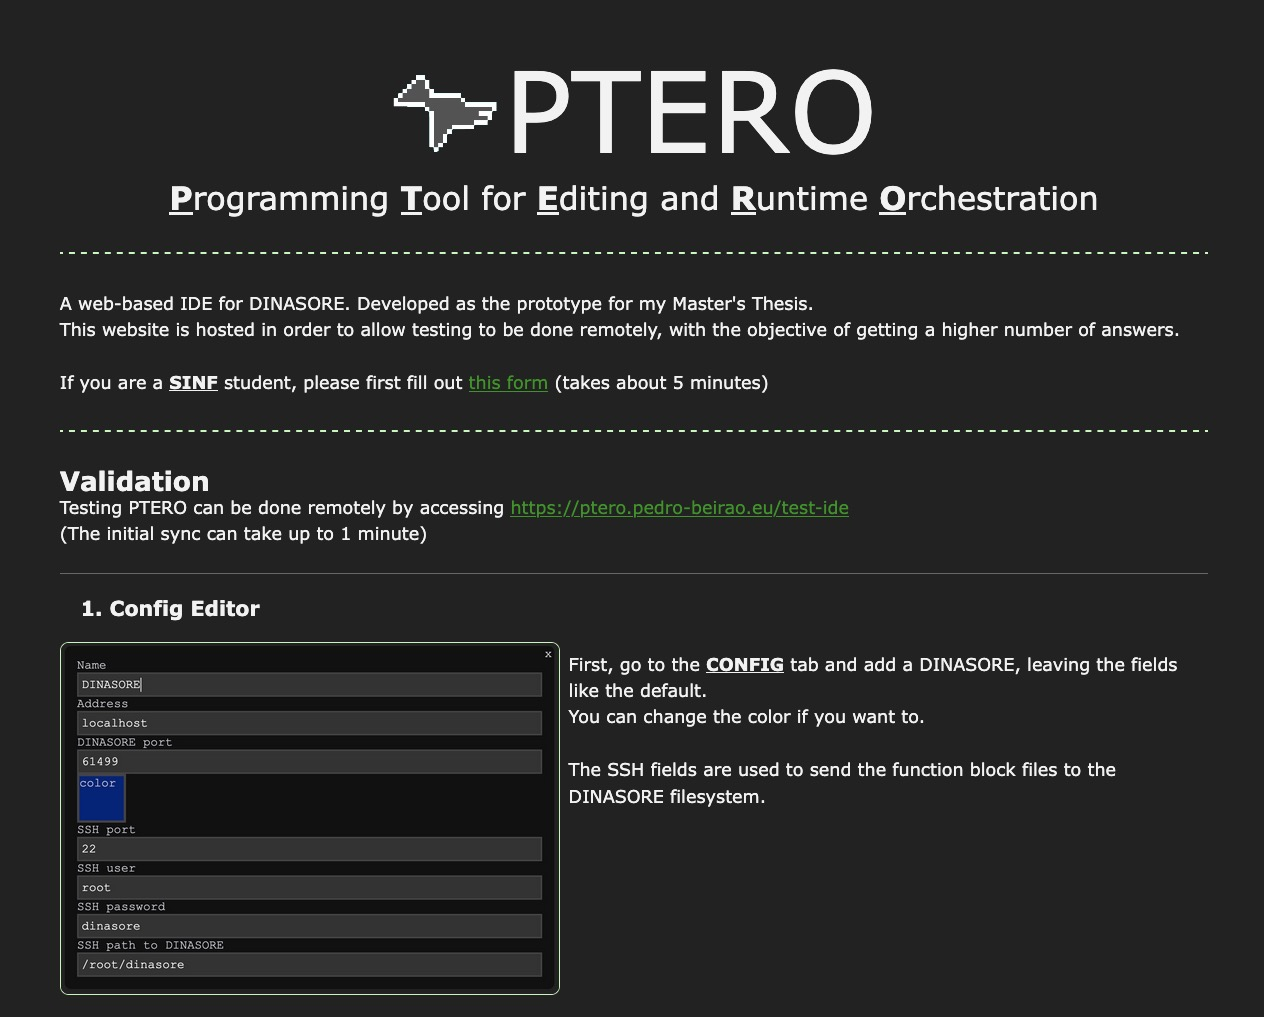
\includegraphics[width=0.9\linewidth]{appendix/1.jpg}
  \caption{Configuration instructions.}
  \label{fig:appendix-1}
\end{figure}

\begin{figure}[H]
  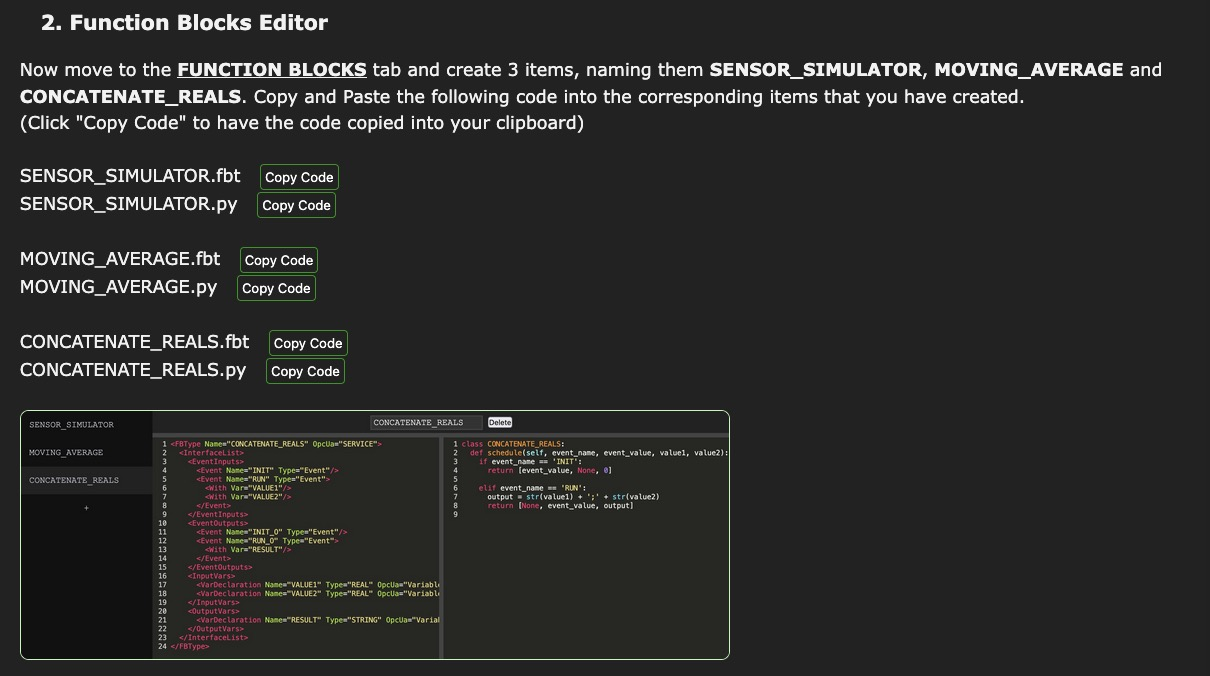
\includegraphics[width=0.9\linewidth]{appendix/2.jpg}
  \caption{Code editing instructions.}
  \label{fig:appendix-2}
\end{figure}

\begin{figure}[H]
  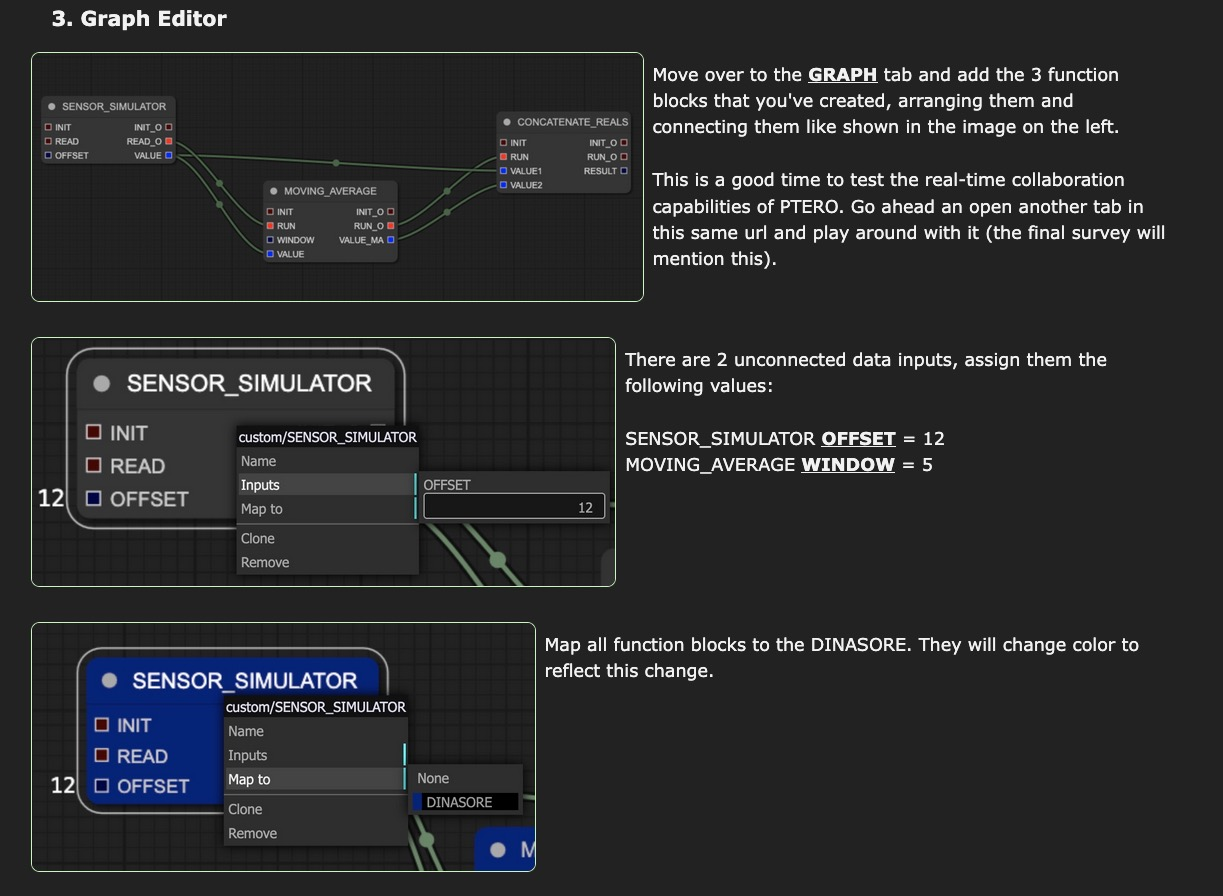
\includegraphics[width=0.9\linewidth]{appendix/3.jpg}
  \caption{Graph instructions.}
  \label{fig:appendix-3}
\end{figure}

\begin{figure}[H]
  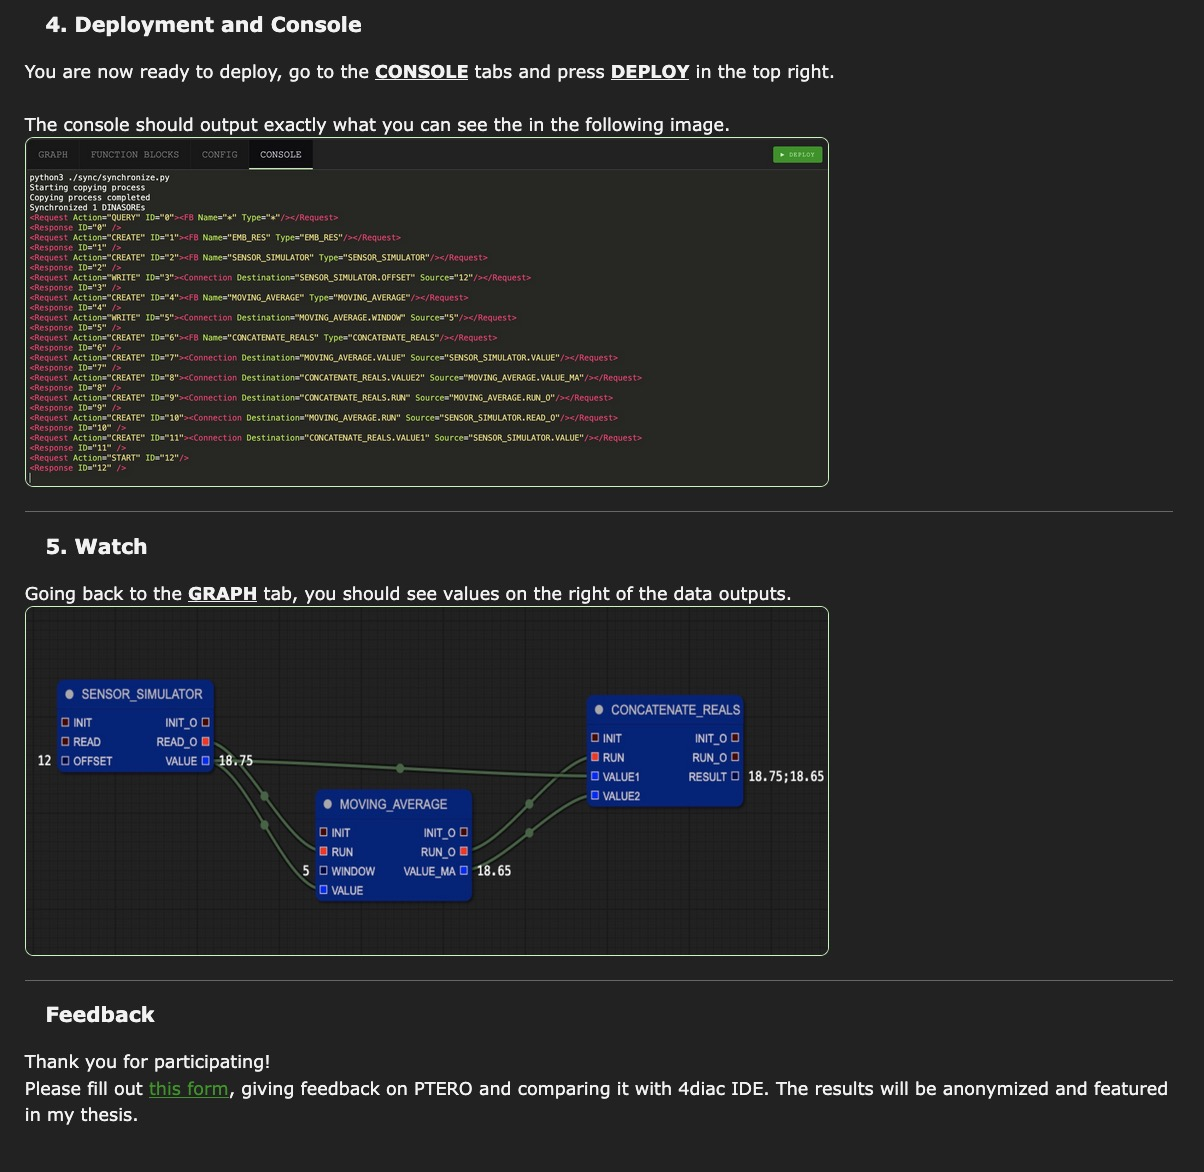
\includegraphics[width=0.9\linewidth]{appendix/4.jpg}
  \caption{Deployment and monitoring instructions.}
  \label{fig:appendix-4}
\end{figure}


\end{document}
